\documentclass[a4paper]{article}

%--------------------------------------------------------------------------
\usepackage[a4paper, total={6in, 9in}]{geometry}
\usepackage{amsmath}
\usepackage{booktabs}
\usepackage{caption}
\usepackage{graphicx}
\usepackage{float}
\usepackage{inconsolata}
\usepackage{listings}
\usepackage{xcolor}
\usepackage{siunitx}
\usepackage[most]{tcolorbox}
\usepackage{etoolbox}

\makeatletter
\patchcmd{\l@section}
{\hfil}
{\leaders\hbox{\normalfont$\m@th\mkern \@dotsep mu\hbox{.}\mkern \@dotsep mu$}\hfill}
{}{}
\makeatother

%--------------------------------------------------------------------------
\graphicspath{{./fig/}}

%--------------------------------------------------------------------------

\definecolor{mGreen}{rgb}{0,0.6,0}
\definecolor{mGray}{rgb}{0.5,0.5,0.5}
\definecolor{mPurple}{rgb}{0.58,0,0.82}
\definecolor{backgroundColour}{rgb}{0.95,0.95,0.92}

\lstdefinestyle{CStyle}{
	backgroundcolor=\color{backgroundColour},   
	commentstyle=\color{mGreen},
	keywordstyle=\color{magenta},
	numberstyle=\tiny\color{mGray},
	stringstyle=\color{mPurple},
	basicstyle=\footnotesize,
	breakatwhitespace=false,         
	breaklines=true,                 
	captionpos=b,                    
	keepspaces=true,                 
	numbers=left,                    
	numbersep=5pt,                  
	showspaces=false,                
	showstringspaces=false,
	showtabs=false,                  
	tabsize=2,
	language=C
}

\setlength\parindent{0pt}

%--------------------------------------------------------------------------
\begin{document}
\title{HIT332: Embedded and Mobile Systems\\ Practical 2 Notes}
\author{Shane Reynolds}
\maketitle

\tableofcontents

%--------------------------------------------------------------------------
\section{Introduction \& Background}
The intention behind this brief set of notes is to provide guidance on how well the practicals and projects for HIT332: Embedded and Mobile Systems achieve their intended outcomes. There are 5 practicals in total, and 3 projects. This set of notes will cover Practical 2. The practicals (and projects) make use of a development board created by Damien Hill and Ben Saunders of Charles Darwin University. The main component of the board is the Atmel ATmega1281 16au 16MHz, 8-bit microcontroller. The development board can be seen in Figure 1.

\begin{figure}[h]
	\centering
	\frame{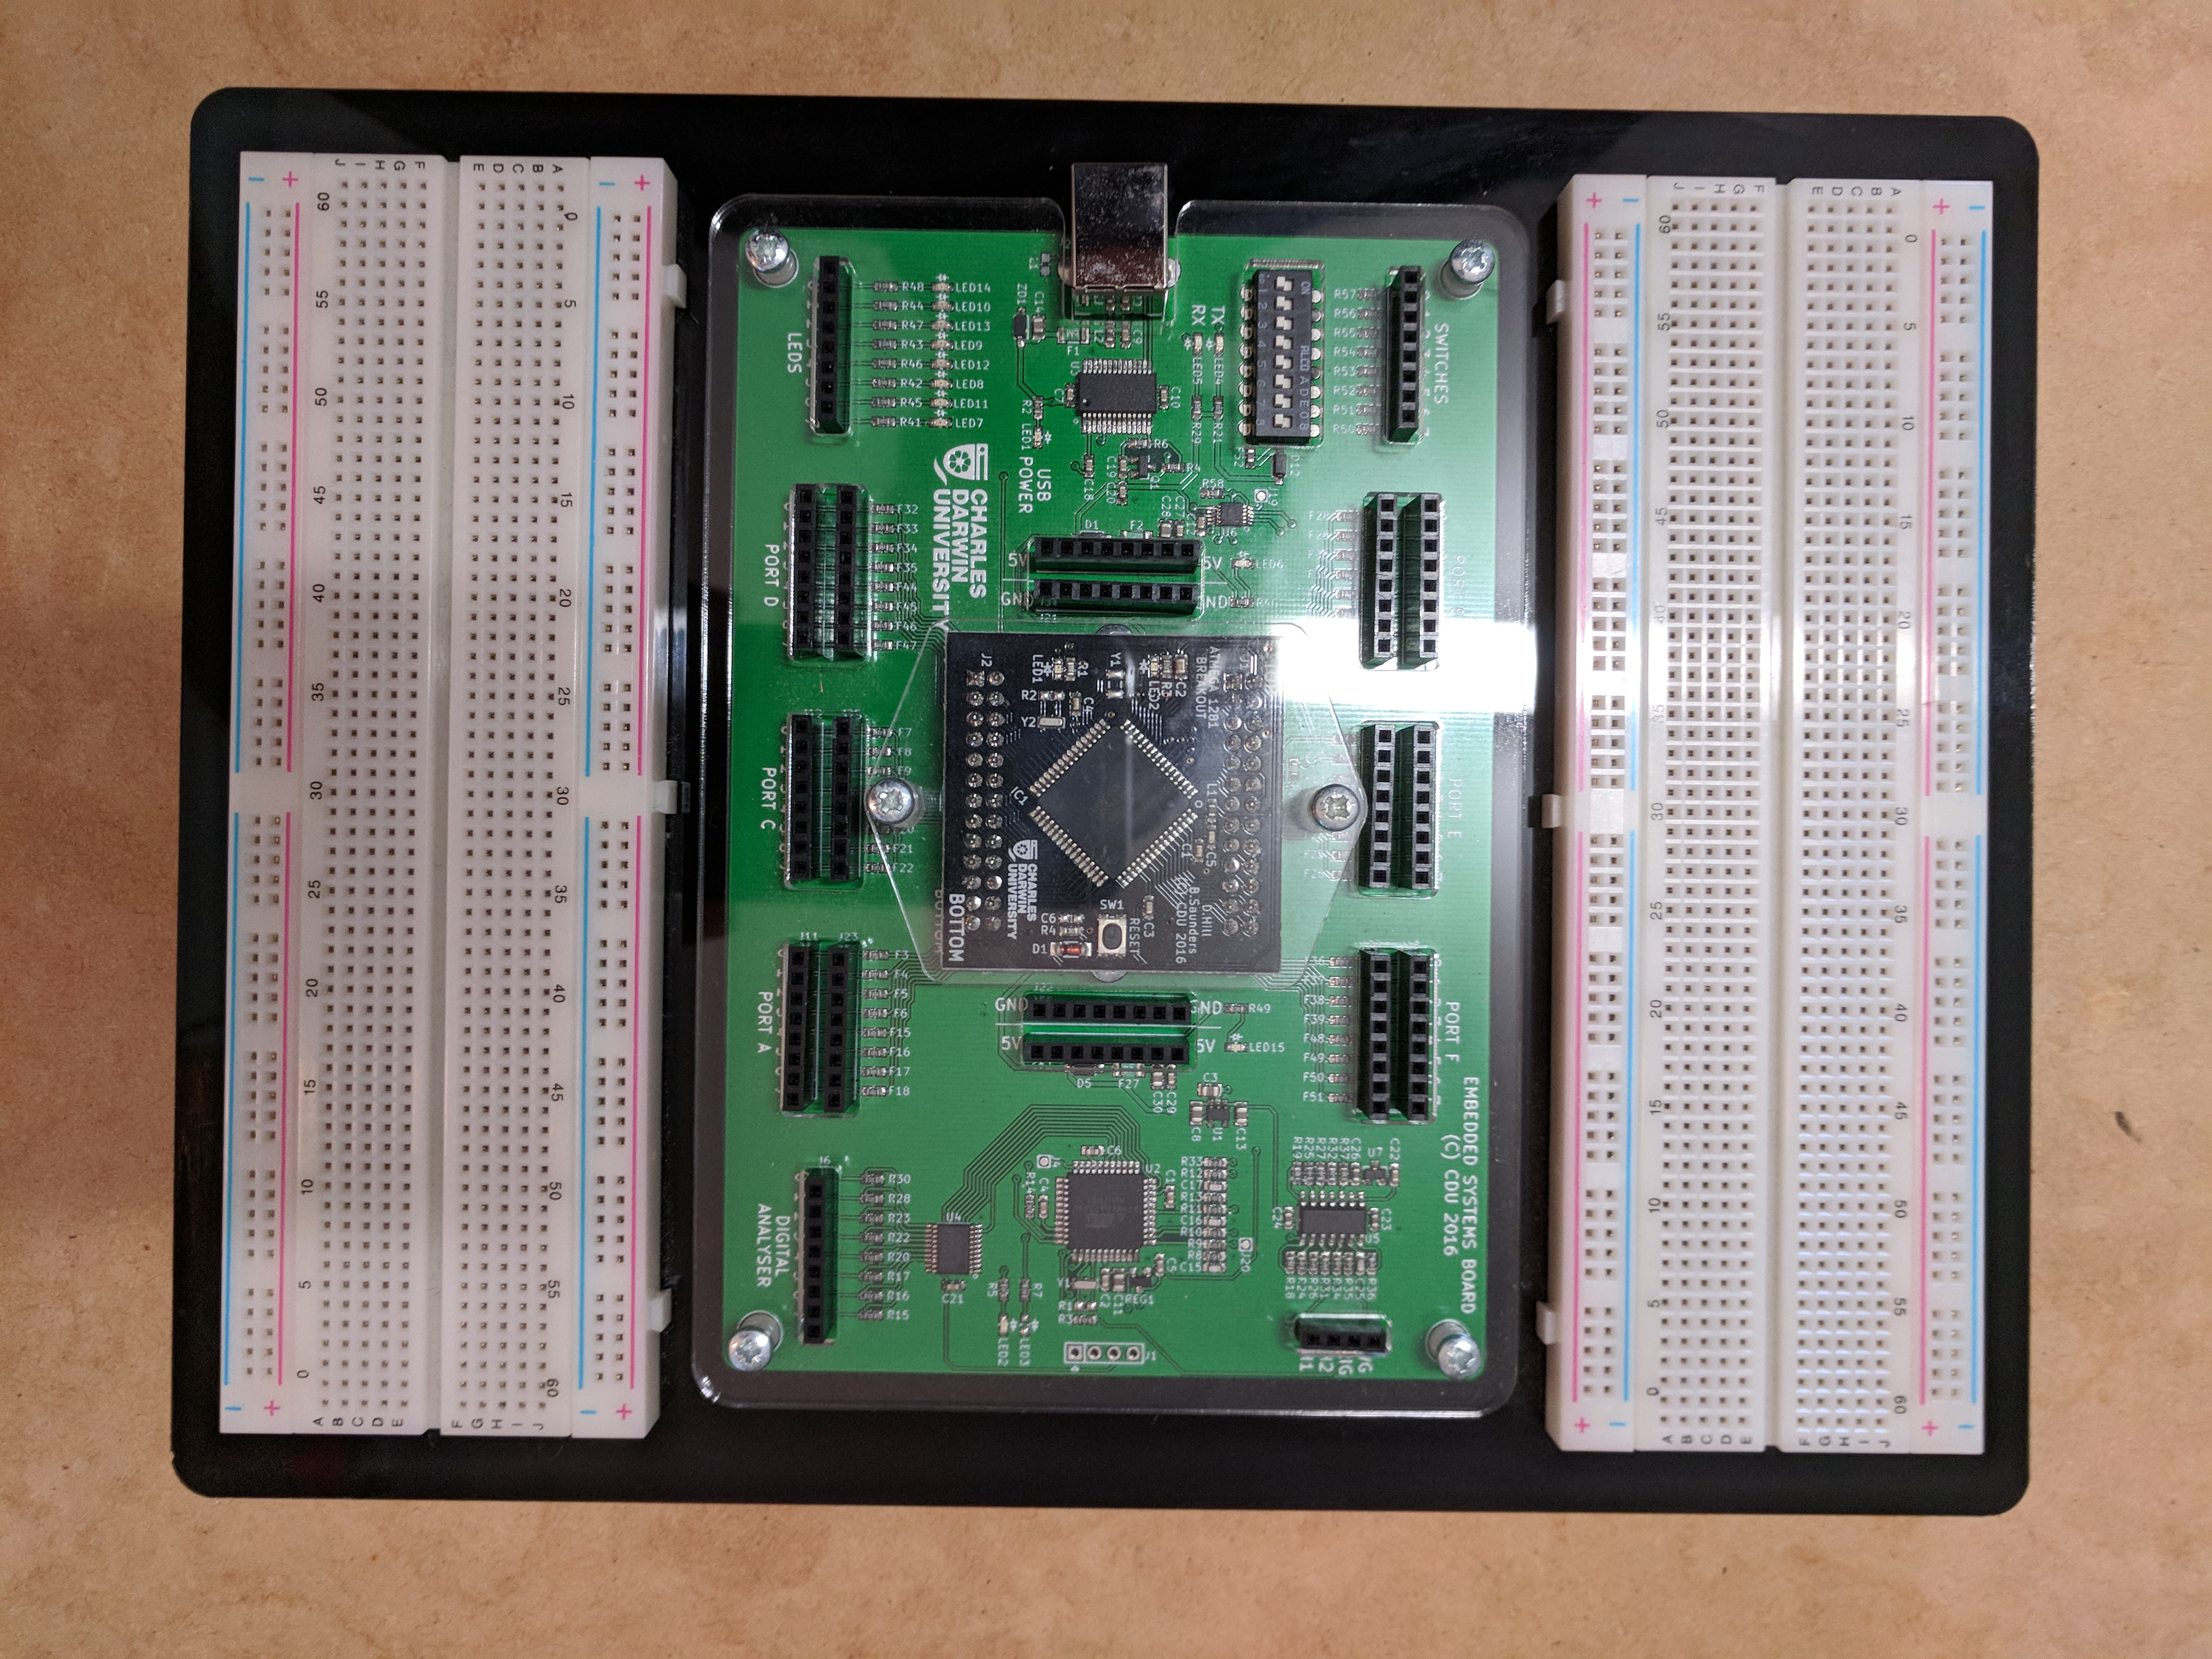
\includegraphics[scale=0.05]{fig1}}
	\caption{The development board which is used in practicals and projects for HIT332: Embedded and Mobile Systems}
\end{figure}

It must be highlighted that these notes have been developed using the board outside of its intended ecosystem. The board is made to be used on CDU's Casuarina Campus in one of the Engineering computer labs. These labs have the appropriate software installed in the correct file paths. These notes have been written using software installed on a personal machine which CDU does not control. Furthermore, the components (other than the development board) used to complete the exercises were sourced independently from a local electronics supplier, independently of CDU. The notes will be highlighted where there has been a significant departure from the intended experience.

\section{Connecting to the USB and Installing the Driver}
Connecting the development board to USB installed the driver as indicated in the instructions. The only point of difference was that the COM3 port was specified for the connection, as opposed to COM15, however, this behaviour is acknowledged in the practical instructions.

\section{Checking out the Hardware}
The LEDs were connected to the 5$\si{\volt}$ supply and worked as intended - this can be seen in Figure 2. Further, the LEDs were connected to the 5$\si{\volt}$ dip switches, which also worked as intended, shown in Figures 3 and 4.

\begin{figure}[h]
	\centering
	\frame{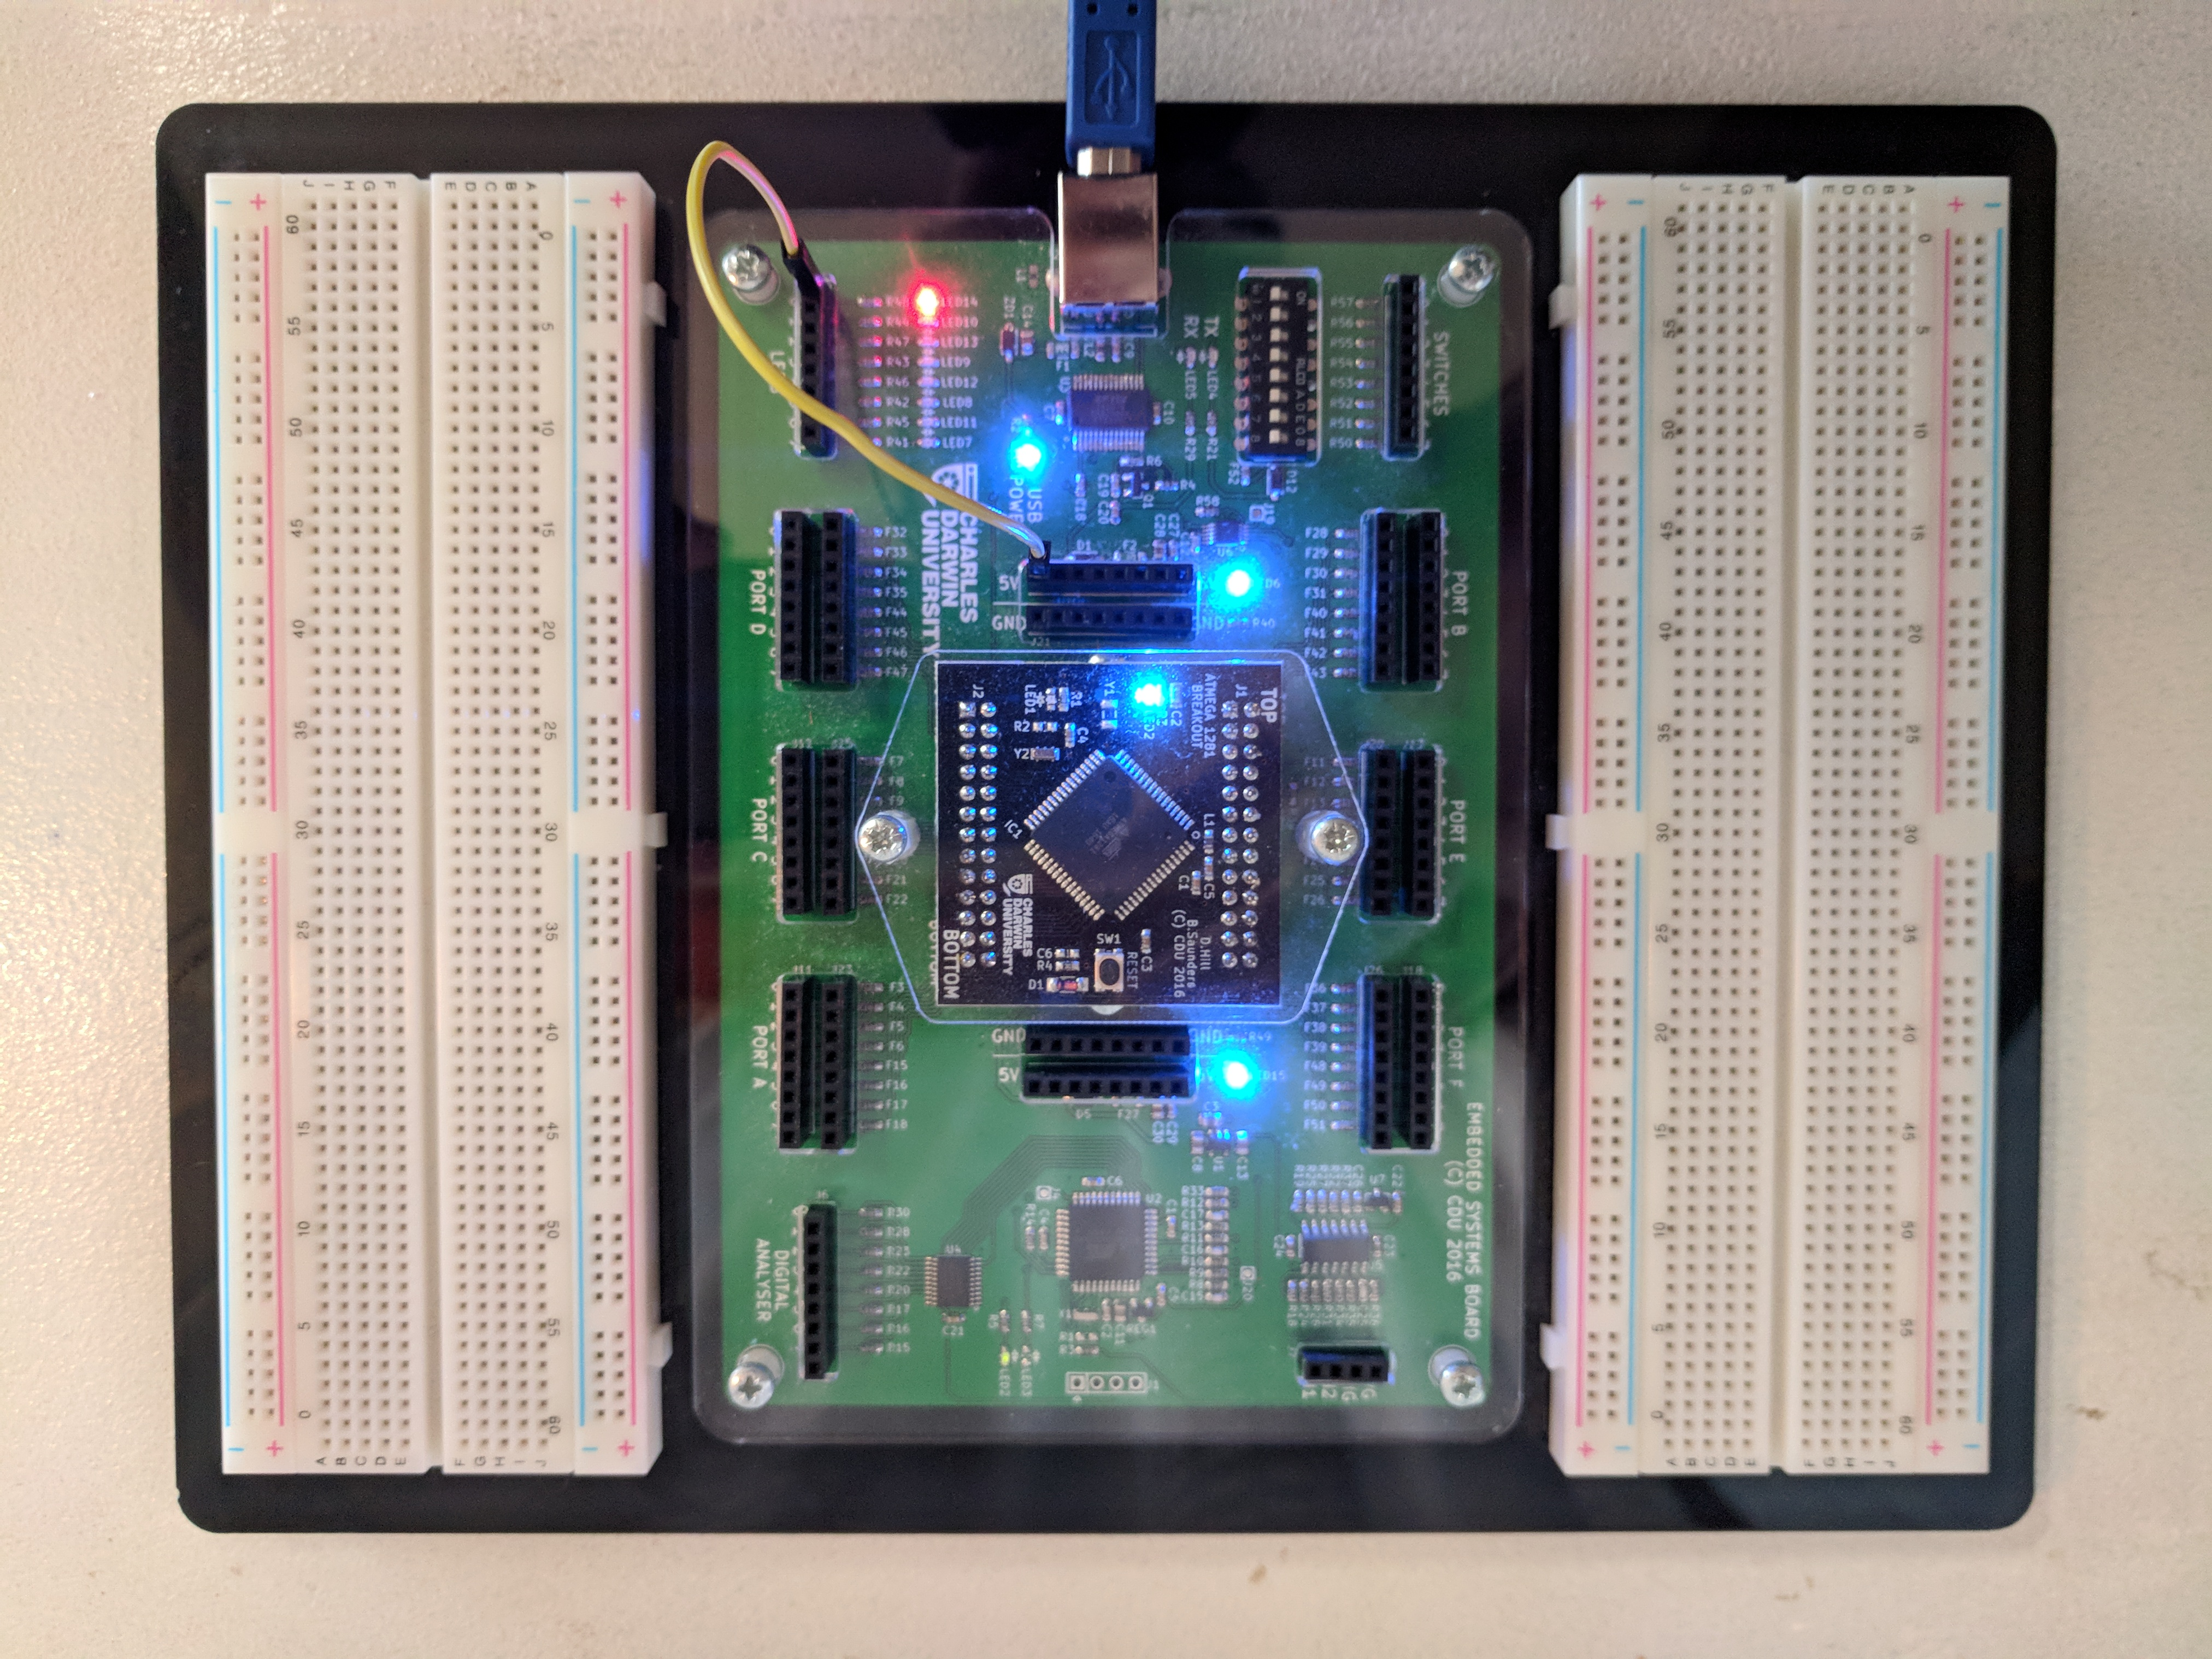
\includegraphics[scale=0.05]{fig2}}
	\caption{Five volts supplied to LED.}
\end{figure}

\section{Writing the source code}
The launch editor button located on the CDU Toolbox Lanucher did not work since Notepad++ was located in a different file path to the one implemented in the launcher. This was expected behaviour given the intended ecosystem is not being used. The instructions for using Notepad++ were fit for purpose, and the \verb|main.c| developed can be seen in Figure 5.

\begin{figure}[h]
\begin{lstlisting}[style=CStyle]
#include <avr/io.h>

int main (void){
DDRD = 0xFF;
PORTD = 0xAA;
while(1){}
}
\end{lstlisting}
\caption{The implementation of the Hello, world! introductory program in \texttt{main.c}}
\end{figure}

\begin{figure}[h]
	\centering
	\begin{minipage}[t]{0.45\textwidth}
		\centering
		\frame{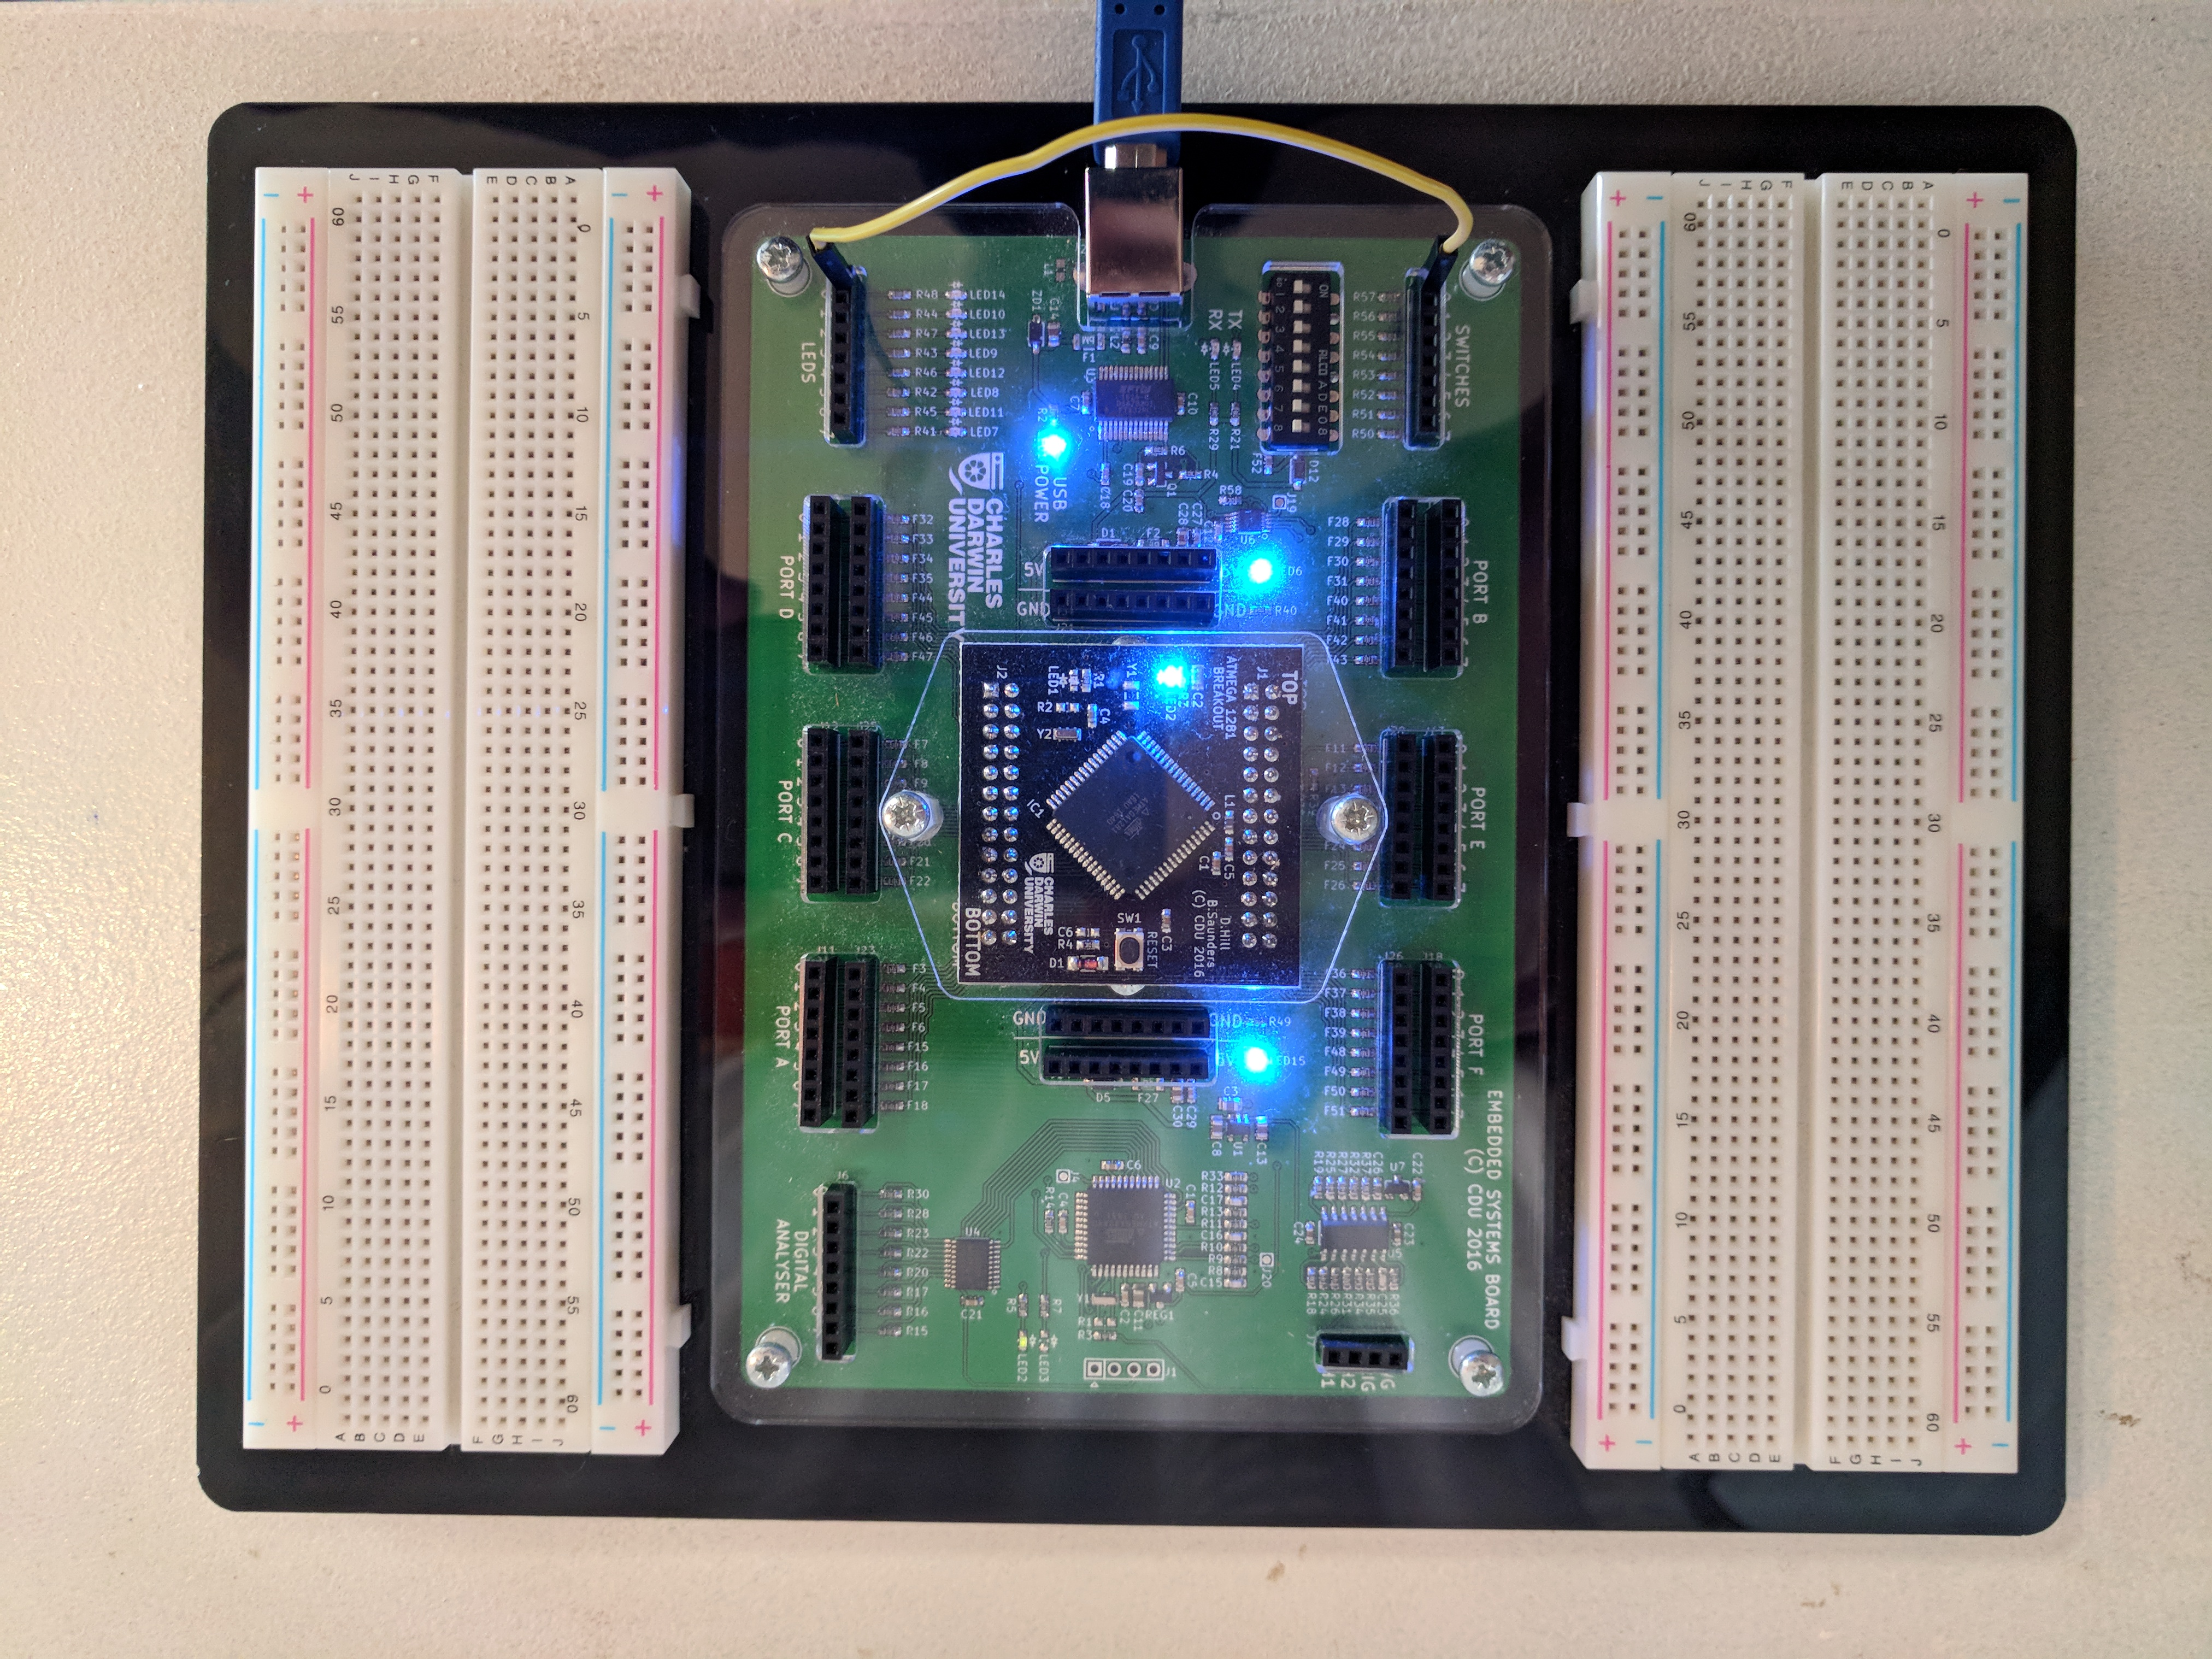
\includegraphics[scale=0.04]{fig3}}
		\caption{Dip switch in the off position, LED is off.}
	\end{minipage}
	\hspace{1cm}
	\begin{minipage}[t]{0.45\textwidth}
		\centering
		\frame{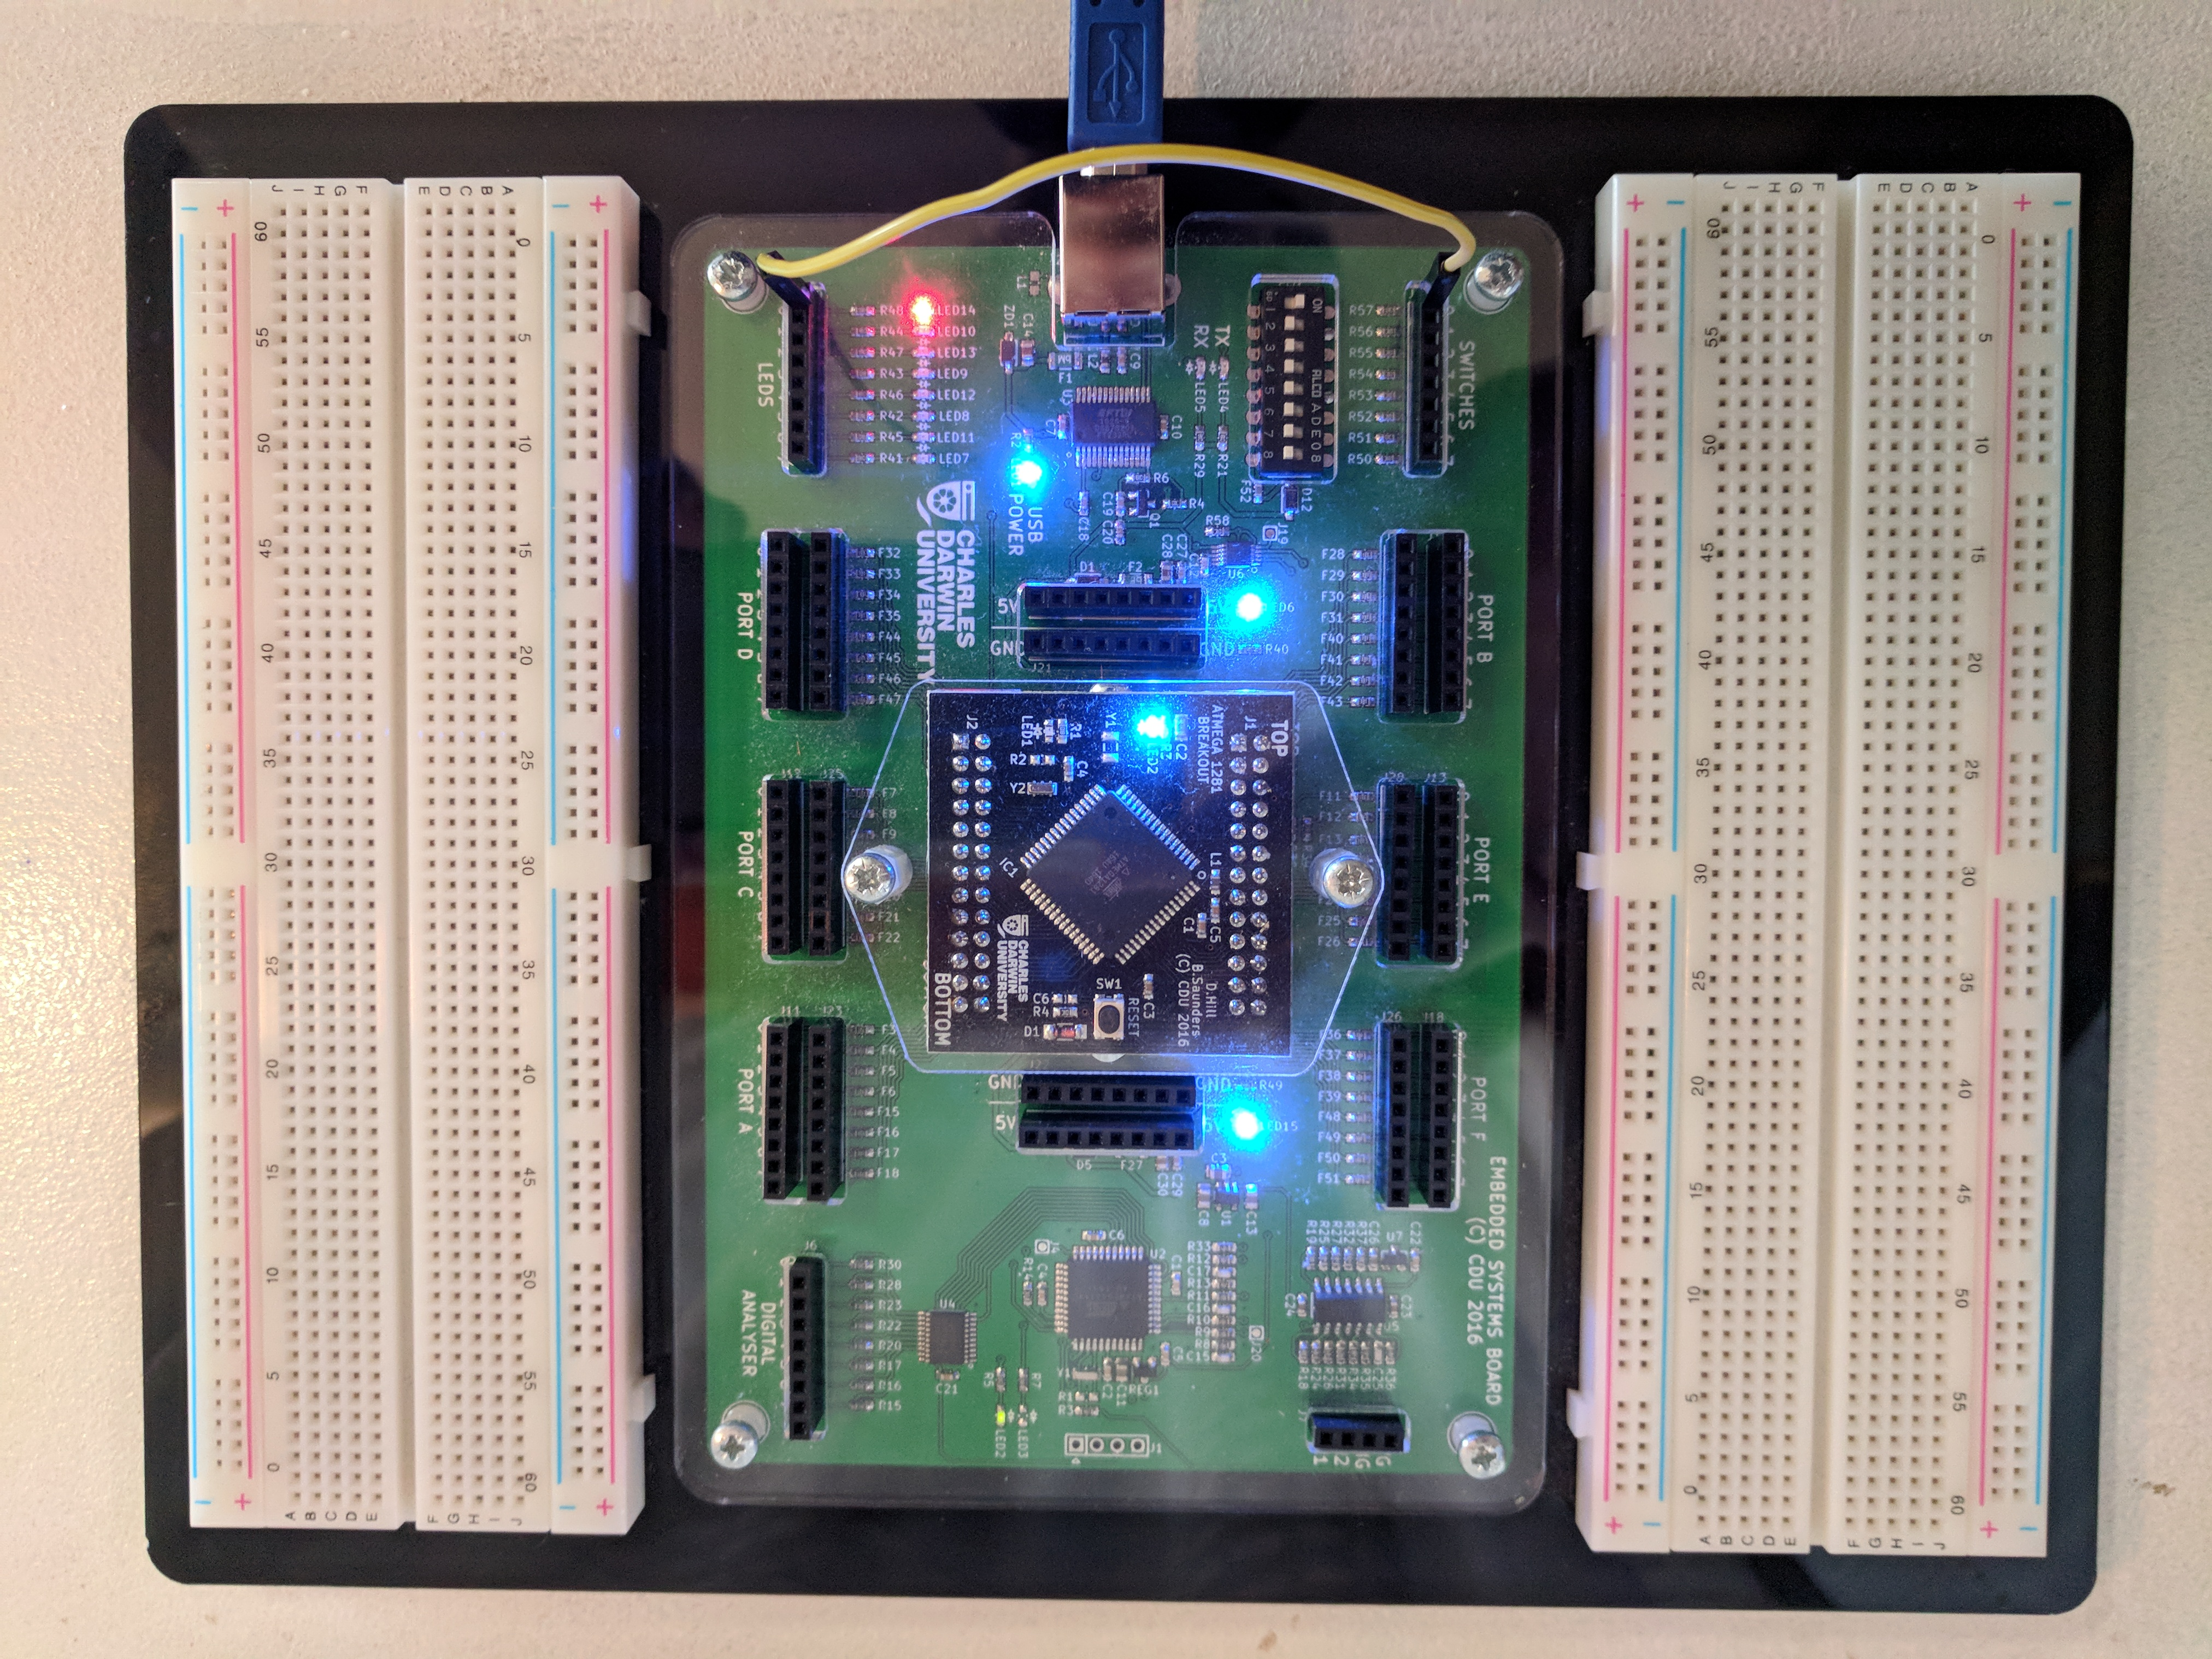
\includegraphics[scale=0.04]{fig4}}
		\caption{Dip switch in the on position, LED is on.}
	\end{minipage}
\end{figure}

\section{Compiling and Linking}
Problems were encountered using the instructions for compiling and linking. This was due to the practical instructions assuming a specific file path for the \verb|avr-gcc| command, and was expected. The use of the commands were tried in both the cmd environment and git bash which is a shell environment provided when installing the Windows version of git. To get around the issues encountered, the full file path to \verb|avr-gcc| was used to access the command. This became time consuming and a short cut using an alias specified in the \verb|.bash_profile| was created. The alias can be seen below:
\begin{center}
	\scriptsize\verb|alias avr_gcc="/c/Users/Shane\ Reynolds/Documents/CDU_embeddedSystems/CDUEmbeddedToolbox/avr_tools/bin/avr-gcc.exe"|
\end{center}


\normalsize This alias allowed the command to be called with the required arguments for compiling and linking.

\section{Creating HEX and Programming the Processor}
The same problems seen in Section 5 were encountered when trying to create hex and program the processor. To get around this more aliases were implemented in \verb|.bash_profile|. The alias for \verb|avr-objcopy| was:
\begin{center}
	\scriptsize\verb|alias avr_objcopy="/c/Users/Shane\ Reynolds/Documents/CDU_embeddedSystems/CDUEmbeddedToolbox/avr_tools/bin/avr-objcopymake.exe"|
\end{center}


The alias for \verb|avr-dude| was as follows:
\begin{center}
	\scriptsize\verb|alias avr_dude="/c/Users/Shane\ Reynolds/Documents/CDU_embeddedSystems/CDUEmbeddedToolbox/avr_tools/bin/avr-dude.exe"|
\end{center}

Once the ATmega1281 was programmed, and the pins were connected to the required LED, the device performed as expected - seen in Figure 6.

\begin{figure}[h]
	\centering
	\frame{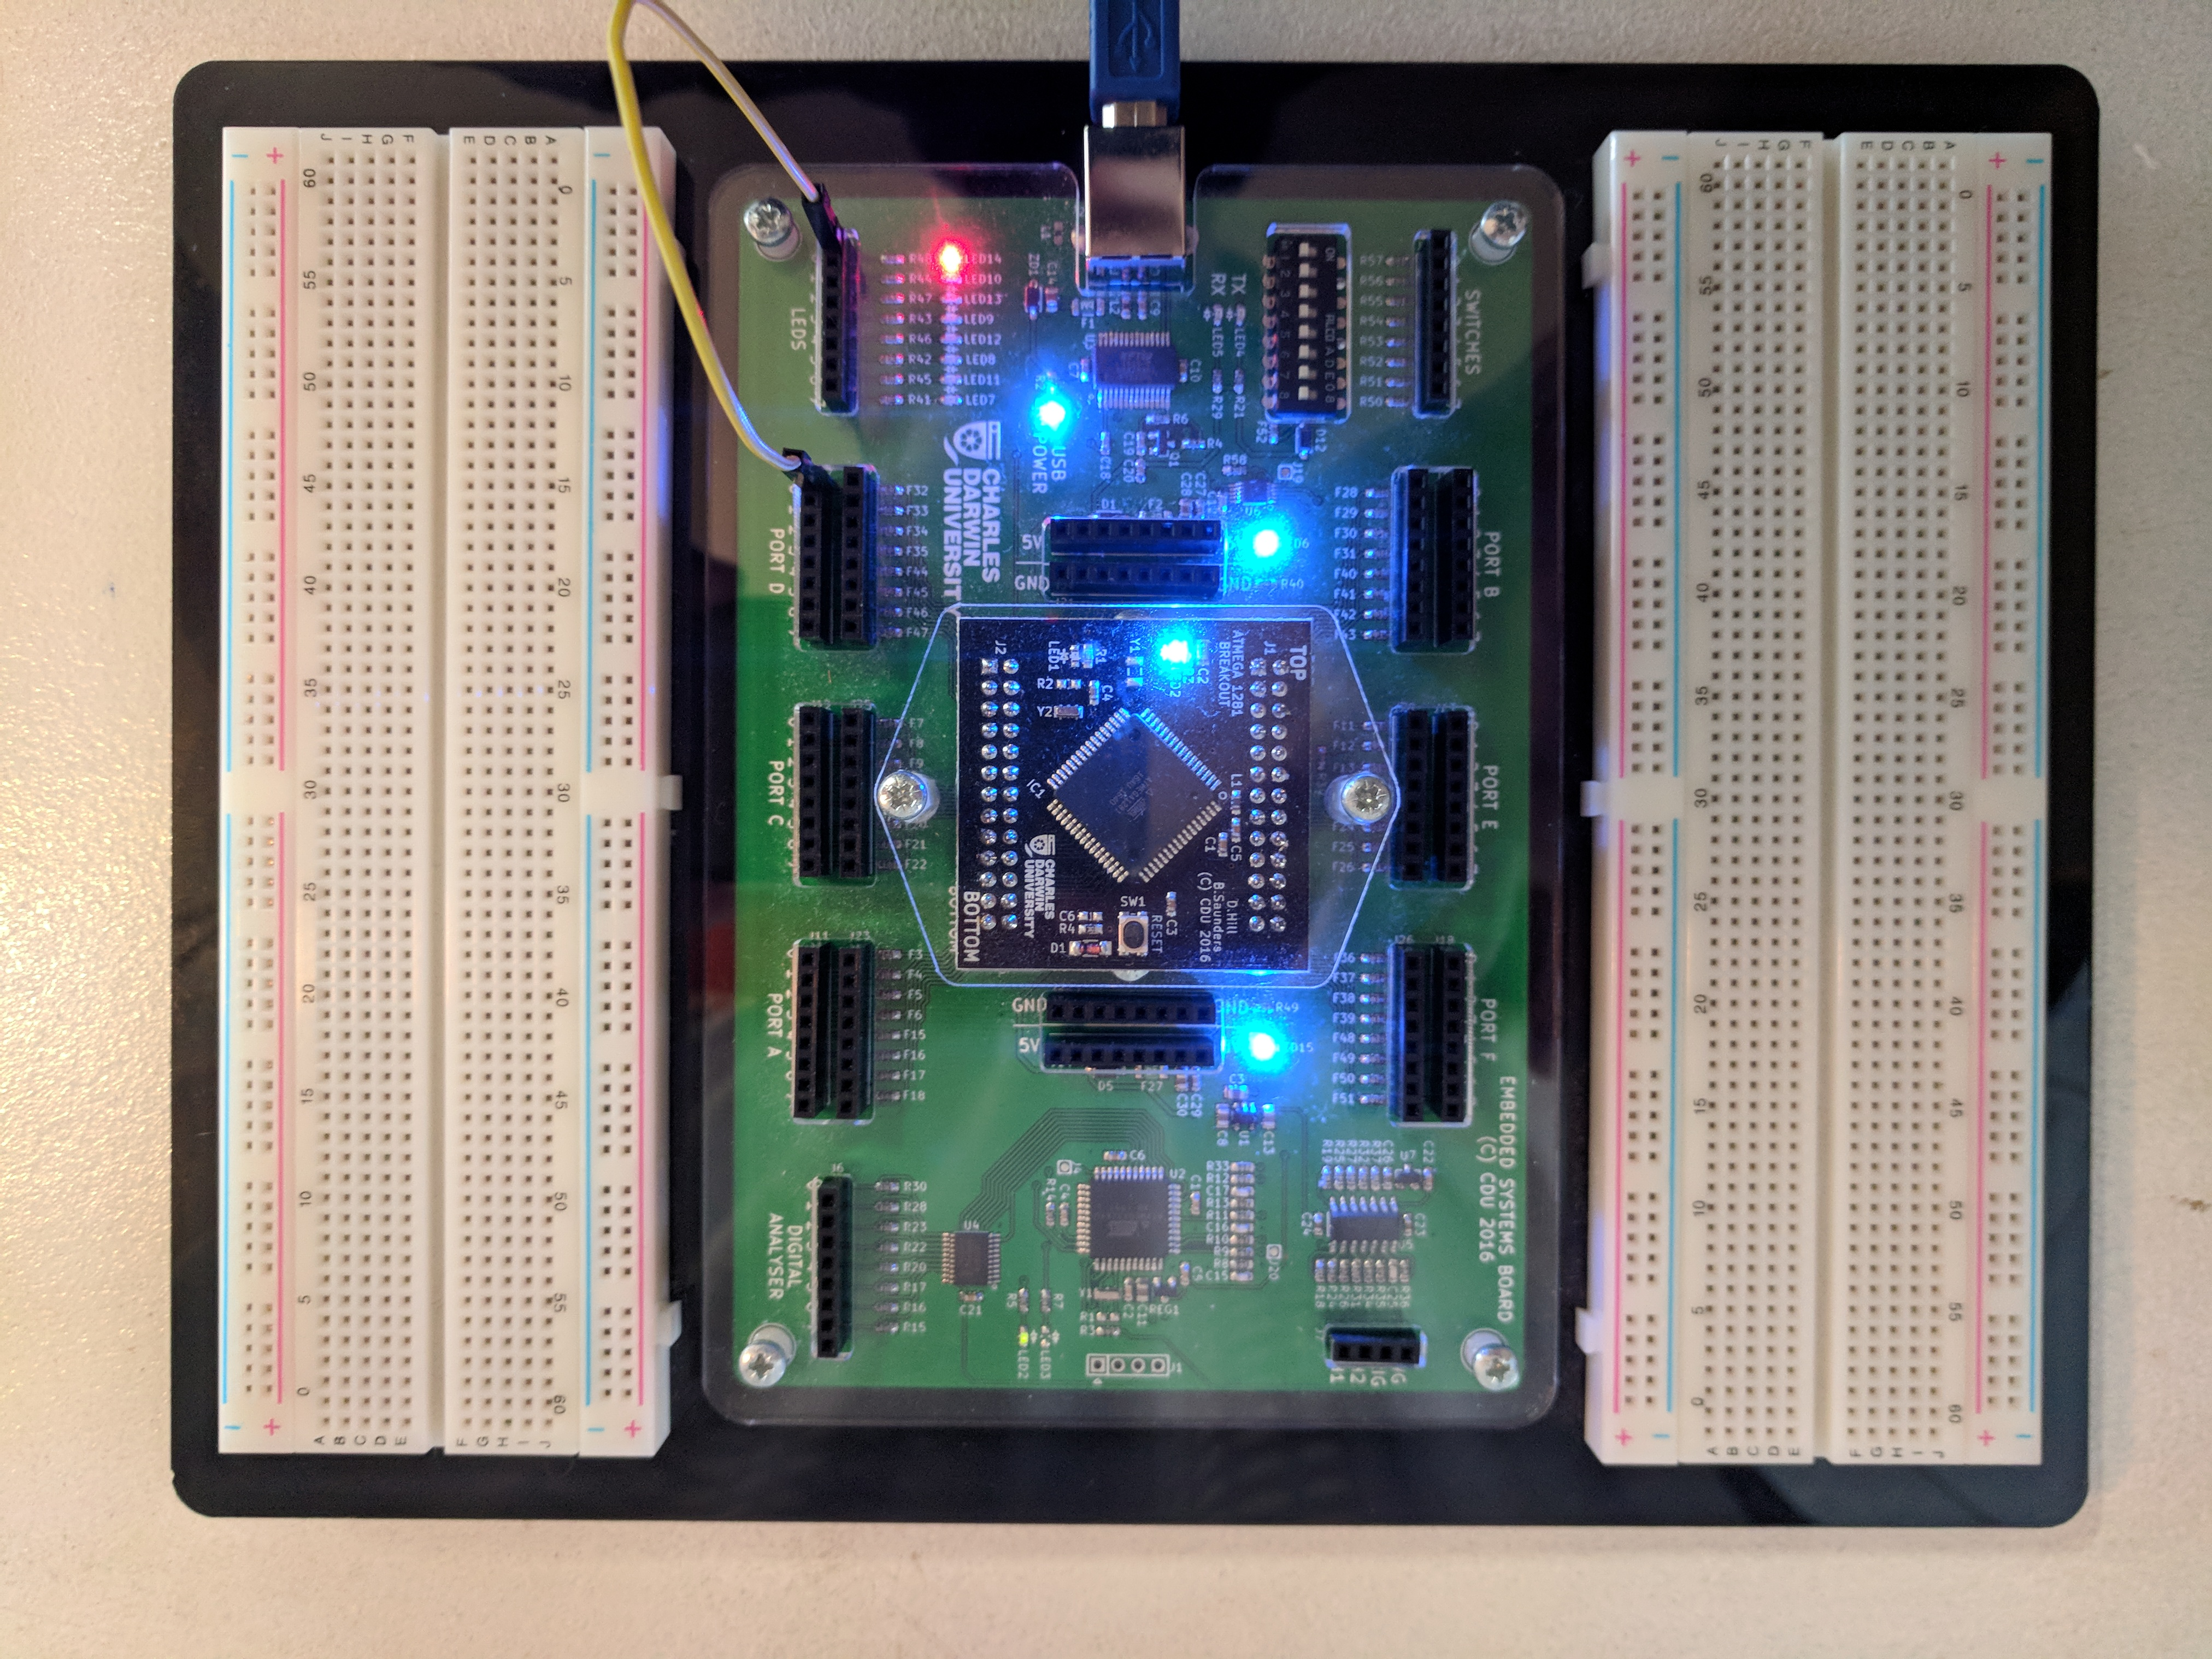
\includegraphics[scale=0.04]{fig5}}
	\caption{ATmega1281 programmed with \texttt{main.c} which places a high on pin 0 for PORTD.}
\end{figure}

\end{document}